\documentclass[aspectratio=169,12pt]{beamer}
\usepackage{fontspec}
\usepackage{amsmath,amssymb,booktabs,array,tabularx,tikz}
\usetikzlibrary{arrows.meta,positioning,fit,shapes.geometric}
\defaultfontfeatures{Ligatures=TeX}
\setmainfont[Path={fonts/TH Sarabun PSK V-1/TH Sarabun PSK V-1/},Extension=.ttf,
  UprightFont={*},BoldFont={* Bold},ItalicFont={* Italic},BoldItalicFont={* BoldItalic}]{THSarabun}
\setsansfont[Path={fonts/TH Sarabun PSK V-1/TH Sarabun PSK V-1/},Extension=.ttf,
  UprightFont={*},BoldFont={* Bold},ItalicFont={* Italic},BoldItalicFont={* BoldItalic}]{THSarabun}
\usefonttheme{professionalfonts}
\definecolor{navy}{HTML}{17365D}
\definecolor{blue}{HTML}{2F75B5}
\definecolor{cyan}{HTML}{00A6A6}
\definecolor{green}{HTML}{2E8B57}
\definecolor{orange}{HTML}{E67E22}
\definecolor{red}{HTML}{C0392B}
\definecolor{light}{HTML}{F3F6FA}
\setbeamercolor{normal text}{fg=navy,bg=white}
\setbeamercolor{frametitle}{fg=white,bg=navy}
\setbeamercolor{title}{fg=white}
\setbeamercolor{subtitle}{fg=white}
\setbeamercolor{structure}{fg=blue}
\setbeamercolor{block title}{fg=white,bg=blue}
\setbeamercolor{block body}{fg=navy,bg=light}
\setbeamercolor{alertblock title}{fg=white,bg=orange}
\setbeamercolor{alertblock body}{fg=navy,bg=orange!8}
\setbeamertemplate{navigation symbols}{}
\setbeamertemplate{itemize item}{\color{cyan}$\blacktriangleright$}
\setbeamertemplate{itemize subitem}{\color{blue}$\bullet$}
\setbeamertemplate{footline}{%
  \leavevmode\hbox{\begin{beamercolorbox}[wd=.84\paperwidth,ht=2.5ex,dp=1.1ex,leftskip=1em]{author in head/foot}%
  \color{navy}\scriptsize Proposed method -- ยังไม่ใช่ผล production
  \end{beamercolorbox}\begin{beamercolorbox}[wd=.16\paperwidth,ht=2.5ex,dp=1.1ex,center]{date in head/foot}%
  \color{navy}\scriptsize\insertframenumber/\inserttotalframenumber
  \end{beamercolorbox}}}
\setbeamerfont{normal text}{size=\fontsize{17}{20}}
\setbeamerfont{frametitle}{size=\fontsize{24}{27},series=\bfseries}
\setbeamerfont{title}{size=\fontsize{30}{34},series=\bfseries}
\setbeamerfont{subtitle}{size=\fontsize{20}{24}}
\setbeamerfont{block title}{size=\fontsize{17}{20},series=\bfseries}
\setbeamerfont{block body}{size=\fontsize{16}{19}}
\setlength{\leftmargini}{1.25em}
\newcommand{\proposal}{\textcolor{orange}{\textbf{PROPOSED}}}
\newcommand{\verified}{\textcolor{green}{\textbf{VERIFIED CURRENT}}}
\newcommand{\gate}[1]{\tikz[baseline=-0.5ex]\node[rounded corners=2pt,fill=green!12,draw=green,inner xsep=4pt,inner ysep=1pt]{#1};}

\title{Adaptive System-Level GFL/GFM Switching}
\subtitle{Event-triggered finite-control-set\newline predictive supervisor\newline
สำหรับ IEEE 14-bus: 1 SG + 4 IBR}
\author{แนวทางพัฒนาต่อจาก AGSI++ local switching}
\date{4 สิงหาคม 2569}

\begin{document}

\begin{frame}[plain]
  \begin{tikzpicture}[remember picture,overlay]
    \fill[navy] (current page.south west) rectangle (current page.north east);
    \fill[cyan] (current page.south west) rectangle ([xshift=.18\paperwidth]current page.north west);
    \draw[white,opacity=.18,line width=1.2pt] ([xshift=.22\paperwidth,yshift=-.15\paperheight]current page.north west)
      -- ([xshift=.92\paperwidth,yshift=-.15\paperheight]current page.north west);
  \end{tikzpicture}
  \vspace{1.15cm}
  \hspace{1.4cm}\begin{minipage}{.78\textwidth}
    {\usebeamerfont{title}\color{white}\inserttitle\par}
    \vspace{.3cm}
    {\usebeamerfont{subtitle}\color{white}\insertsubtitle\par}
    \vspace{.75cm}
    {\color{white!85}\insertauthor\par\insertdate}
  \end{minipage}
\end{frame}

\begin{frame}{1. Feedback ที่ต้องตอบให้ตรงประเด็น}
\begin{columns}[T,onlytextwidth]
\column{.48\textwidth}
\begin{alertblock}{ข้อจำกัดของวิธีปัจจุบัน}
AGSI++ เป็นดัชนีความเครียด \emph{ราย IBR} แล้วใช้ threshold, hysteresis และ dwell สั่ง state machine
\end{alertblock}
\begin{itemize}
  \item มี $V,f,\mathrm{RoCoF},P,SCR,v_q,GRA$ แต่เป็นข้อมูล local
  \item ไม่ได้เลือกจากผลกระทบต่อโครงข่ายทั้งระบบ
  \item เมื่อถึงเกณฑ์จึงเปลี่ยนโหมดตามกฎที่ออกแบบไว้ล่วงหน้า
\end{itemize}
\column{.48\textwidth}
\begin{block}{คำถามวิจัยใหม่}
ก่อนสลับ เราจะรู้ได้อย่างไรว่า \textbf{ควรสลับตัวใด กี่ตัว และใครเป็น reference leader} เพื่อให้ระบบโดยรวมปลอดภัยที่สุด?
\end{block}
\vspace{.25cm}
\centering
\proposal\quad เพิ่ม adaptive system-level supervisor เหนือ AGSI++
\end{columns}
\end{frame}

\begin{frame}{2. แยกให้ชัด: ของที่มีแล้วกับของที่จะพัฒนา}
\begin{tabularx}{\textwidth}{>{\bfseries}p{.23\textwidth}XX}
\toprule
ชั้นควบคุม & สถานะปัจจุบัน & งานที่จะเพิ่ม \\
\midrule
Local indicator & AGSI++ คำนวณ stress ราย IBR & ใช้เป็น event trigger และข้อมูลประกอบ \\
Local state machine & GFL/GFM, threshold, dwell, hysteresis & คงไว้เป็น safety interlock \\
Reference transaction & SG-trip override และ SG handback & ให้ supervisor เลือก leader/ชุด GFM \\
System decision & ยังไม่มีการเปรียบเทียบ mode ทั้งระบบ & ประเมิน candidate จาก full-network state \\
Prediction & ไม่มี look-ahead ก่อน commit & จำลอง candidate ช่วงสั้นก่อนเลือก \\
\bottomrule
\end{tabularx}
\vspace{.35cm}
\begin{block}{ขอบเขตงานรอบถัดไป}
พัฒนา logic การเลือกโหมดเท่านั้น; ไม่เพิ่ม AVR, ไม่ใช้ BO/LLM ในวงรอบสั่งสวิตช์ และไม่เปลี่ยนสมการ SG/IBR ที่ตรวจแล้ว
\end{block}
\end{frame}

\begin{frame}[shrink=4]{3. Method คืออะไร?}
\begin{block}{ชื่อที่เสนอ}
\textbf{Event-Triggered Finite-Control-Set Predictive Supervisor (ET-FCSPS)}
\end{block}
\begin{columns}[T,onlytextwidth]
\column{.31\textwidth}
\centering\textcolor{cyan}{\Large Event-triggered}\par
\small ทำงานเมื่อ AGSI/event/topology เปลี่ยน ไม่ค้นหาทุก integration step
\column{.31\textwidth}
\centering\textcolor{blue}{\Large Finite control set}\par
\small ตัวเลือกเป็น binary mode vector ที่แจกแจงได้ครบ ไม่ต้องหา optimum บน space ต่อเนื่อง
\column{.31\textwidth}
\centering\textcolor{orange}{\Large Predictive}\par
\small ใช้แบบจำลองโครงข่ายทำนายผลช่วงสั้นก่อน commit คำสั่งจริง
\end{columns}
\vspace{.45cm}
\centering
\Large AGSI++ ``ขอพิจารณาสลับ'' \quad$\neq$\quad ``สั่งสลับทันที''
\vspace{.25cm}

\small นำแนวคิด finite-action prediction มาปรับใช้ที่ระดับ supervisory mode selection
ไม่ใช่ converter-level semiconductor switching
\end{frame}

\begin{frame}[shrink=8]{4. ตัวแปรตัดสินใจ: 16 mode combinations}
สำหรับ IBR 4 ตัว กำหนด
\[
\mathbf m=[m_1,m_2,m_3,m_4]\in\{0,1\}^4,
\qquad 0=\mathrm{GFL},\;1=\mathrm{GFM}.
\]
\begin{columns}[T,onlytextwidth]
\column{.52\textwidth}
\begin{itemize}
  \item มี candidate ทั้งหมด $2^4=16$ รูปแบบ
  \item ถ้า SG offline เพิ่มตัวแปร owner $r\in\{1,2,3,4\}$
  \item บังคับ $m_r=1$ และมี reference owner เพียงหนึ่งตัว
  \item ตัด candidate ที่ละเมิด dwell/lockout ก่อนจำลอง
\end{itemize}
\column{.44\textwidth}
\begin{block}{ตัวอย่าง}
\begin{tabular}{cl}
$[0000]$ & all GFL \\
$[1000]$ & IBR1 GFM \\
$[1010]$ & IBR1,3 GFM \\
$[1111]$ & all GFM
\end{tabular}
\end{block}
\begin{alertblock}{ไม่ใช่ PF slack}
owner คือ angle/frequency reference ของ island; ทุกอุปกรณ์ยังอยู่ใน full KCL
\end{alertblock}
\end{columns}
\end{frame}

\begin{frame}[shrink=8]{5. Controller ต้องมองอะไรทั้งระบบ?}
\begin{columns}[T,onlytextwidth]
\column{.48\textwidth}
\begin{block}{สถานะโครงข่าย}
\begin{itemize}
  \item $V_{\min},V_{\max}$ และ voltage violation ทุกบัส
  \item topology, island, สายที่เปิด และ electrical distance
  \item line loading และ short-circuit strength
  \item SG/reference availability: $GRA$
\end{itemize}
\end{block}
\column{.48\textwidth}
\begin{block}{สมดุลและ headroom}
\begin{itemize}
  \item frequency/COI frequency และ RoCoF
  \item $\Delta P=P_{gen}-P_{load}-P_{loss}$
  \item $Q$ requirement และ reactive reserve
  \item $P/Q$ headroom, current limit และ energy availability ของ IBR
\end{itemize}
\end{block}
\end{columns}
\vspace{.2cm}
\begin{alertblock}{ข้อควรระวัง}
``กำลังรวม'' ต้องรวม network losses และใช้ sign/base เดียวกัน ไม่ใช่บวกค่า $P$ จากกราฟโดยตรง
\end{alertblock}
\end{frame}

\begin{frame}{6. ลำดับการทำงานของ ET-FCSPS}
\centering
\begin{tikzpicture}[node distance=5mm and 7mm,>=Latex,
box/.style={rounded corners=3pt,draw=blue,thick,fill=light,minimum width=2.3cm,minimum height=1.0cm,align=center},
decision/.style={diamond,aspect=2.1,draw=orange,thick,fill=orange!8,align=center,inner sep=2pt}]
\node[box] (measure) {รับ accepted state\\และ event};
\node[decision,right=of measure] (trigger) {AGSI/event\\trigger?};
\node[box,right=of trigger] (enum) {สร้าง admissible\\candidate set};
\node[box,below=of enum] (screen) {algebraic\\feasibility screen};
\node[box,left=of screen] (predict) {short-horizon\\prediction};
\node[box,left=of predict] (rank) {คำนวณ cost\\และจัดอันดับ};
\node[decision,below=of rank] (feasible) {มี candidate\\ผ่านหรือไม่?};
\node[box,right=of feasible] (commit) {dwell/guard\\atomic commit};
\node[box,right=of commit,draw=red] (fallback) {fail-closed\\safe fallback};
\draw[->,thick] (measure)--(trigger);
\draw[->,thick] (trigger)--node[above]{yes}(enum);
\draw[->,thick] (enum)--(screen);
\draw[->,thick] (screen)--(predict);
\draw[->,thick] (predict)--(rank);
\draw[->,thick] (rank)--(feasible);
\draw[->,thick] (feasible)--node[above]{yes}(commit);
\draw[->,thick] (feasible.south) -- ++(0,-3mm) -| node[pos=.18,below]{no} (fallback.south);
\draw[->,thick] (trigger.south) |- node[pos=.2,right]{no} (measure.south);
\end{tikzpicture}
\par\vspace{.25cm}
{\small ใช้เฉพาะ accepted production states; candidate trial ห้ามแก้ state จริงก่อน transaction commit\par}
\end{frame}

\begin{frame}{7. ชั้นที่ 1: feasibility gates ก่อนจัดอันดับ}
Candidate $c=(\mathbf m,r)$ ต้องผ่านทุก hard constraint:
\begin{align*}
g_{KCL}(c)&:\quad \|F(x,y,c)\|_\infty\le\varepsilon_{KCL},\\
g_V(c)&:\quad V_{min}^{lim}\le |V_b|\le V_{max}^{lim}\quad\forall b,\\
g_I(c)&:\quad |I_i|\le I_{i,max}\quad\forall i,\\
g_R(c)&:\quad P_{reserve},Q_{reserve}\ \text{ไม่ติดลบ},\\
g_{ref}(c)&:\quad \text{ทุก energized island มี reference owner หนึ่งตัว},\\
g_{hyb}(c)&:\quad \text{ไม่ละเมิด dwell, lockout และ state-transfer contract}.
\end{align*}
\begin{alertblock}{หลัก fail-closed}
ถ้าไม่มี candidate ผ่าน ห้ามเลือก ``ตัวที่ cost น้อยที่สุด'' จากชุดที่ผิด constraint; ต้องใช้ safe fallback ที่ประกาศไว้และบันทึกเหตุผล
\end{alertblock}
\end{frame}

\begin{frame}{8. ชั้นที่ 2: prediction และ objective}
สำหรับ candidate ที่ผ่าน gate ทำนายช่วง $T_p$ แล้วคำนวณ
\[
J(c)=w_VJ_V+w_fJ_f+w_RJ_{RoCoF}+w_PJ_{\Delta P}
     +w_QJ_{Q,res}+w_NN_{GFM}+w_SN_{switch}.
\]
\begin{columns}[T,onlytextwidth]
\column{.55\textwidth}
\begin{itemize}
  \item $J_V$: integral/max ของ voltage violation ทั้งระบบ
  \item $J_f,J_{RoCoF}$: frequency security
  \item $J_{\Delta P}$: active-power imbalance รวม losses
  \item $J_{Q,res}$: reactive reserve shortage
\end{itemize}
\column{.41\textwidth}
\begin{itemize}
  \item $N_{GFM}$: ไม่เปิด GFM เกินจำเป็น
  \item $N_{switch}$: ลด chatter/wear
  \item tie-break: residual, reserve margin, index ลำดับ IBR
\end{itemize}
\end{columns}
\begin{block}{Numerical-integrity contract}
นิยาม normalization, weight, horizon และ tie-break ก่อนดูผล; ห้าม tune เพื่อให้ scenario ที่ต้องการชนะ
\end{block}
\end{frame}

\begin{frame}{9. Reference leader และ coordinated transaction}
\begin{columns}[T,onlytextwidth]
\column{.48\textwidth}
\begin{block}{เมื่อ SG trip / $GRA=0$}
\begin{enumerate}
  \item freeze accepted state และสร้าง candidate
  \item เลือก GFM set พร้อม owner $r$
  \item map state ให้ทุก branch
  \item solve right-limit KCL
  \item commit ทั้ง transaction แบบ atomic
\end{enumerate}
\end{block}
\column{.48\textwidth}
\begin{block}{เมื่อ SG จะกลับ}
\begin{enumerate}
  \item restore topology/load ตาม event contract
  \item ตรวจ $\Delta V,\Delta f,\Delta\theta$ ครบ dwell
  \item close SG และ solve right-limit KCL
  \item handback reference แบบ bumpless
  \item ให้ supervisor ประเมิน all-GFL ใหม่
\end{enumerate}
\end{block}
\end{columns}
\vspace{.2cm}
\centering
\textbf{AGSI ไม่ได้ถูกยกเลิก:} เป็น local evidence; transaction coordinator เป็นผู้อนุมัติคำสั่งระดับระบบ
\end{frame}

\begin{frame}[shrink=6]{10. ตัวอย่างการตอบสนองที่คาดหวัง (ยังไม่ใช่ผล)}
\begin{tabularx}{\textwidth}{>{\bfseries}p{.19\textwidth}XXX}
\toprule
เหตุการณ์ & AGSI local & การประเมินระบบ & คำสั่งที่เป็นไปได้ \\
\midrule
no event & ต่ำทุกตัว & voltage/power/reference ผ่าน & คง all-GFL \\
load step เบา & บางตัวสูงขึ้น & reserve ยังเพียงพอ & ไม่สลับ หรือ GFM 1 ตัว \\
fault เฉพาะจุด & IBR ใกล้ fault สูง & ทดสอบตำแหน่งและ voltage support & เลือก GFM ใกล้พื้นที่อ่อน \\
SG trip & $GRA=0$ & island ต้องมี reference & เลือก owner และ GFM set แบบ atomic \\
SG reclose & index อาจยังสูง & sync guard + predicted handback & คืน SG reference แล้วลด GFM \\
\bottomrule
\end{tabularx}
\vspace{.35cm}
\begin{alertblock}{สิ่งที่ต้องพิสูจน์ด้วยการจำลอง}
คำสั่งข้างต้นเป็น design hypothesis; controller อาจเลือกต่างออกไปตามผล feasibility/prediction จริง
\end{alertblock}
\end{frame}

\begin{frame}[shrink=12]{11. ทำไมเหมาะกว่าการใช้ BO เป็น online switcher?}
\small
\begin{tabularx}{\textwidth}{>{\bfseries}p{.22\textwidth}XX}
\toprule
ประเด็น & Bayesian optimisation & ET-FCS predictive supervisor \\
\midrule
โจทย์หลัก & หา optimum ของ expensive black-box objective & เลือก action จาก finite set ภายใต้ state ปัจจุบัน \\
คำตอบต่อ event & อาศัย surrogate/acquisition ที่เรียนจาก samples & ประเมิน admissible actions ที่แจกแจงไว้โดยตรง \\
hard constraints & ต้องออกแบบ constrained BO เพิ่ม & reject candidate ก่อน ranking ได้ชัดเจน \\
traceability & ต้องอธิบาย surrogate และ uncertainty & แสดง gate, prediction และ cost ของทุก candidate \\
ข้อมูลฝึก & ต้องมี evaluations เพียงพอ & ไม่ต้องฝึก model เพิ่ม; ใช้ project plant model \\
ข้อเสีย & exploration และผลขึ้นกับ prior/kernel & computation โตตาม candidate/horizon \\
\bottomrule
\end{tabularx}
\vspace{.25cm}
\begin{block}{ข้อสรุปที่อ้างได้อย่างเป็นธรรม}
ไม่ได้ ``ดีกว่า BO ทุกกรณี'' แต่เหมาะกว่ากับ decision set 16 รูปแบบที่ต้อง deterministic, constraint-aware และ audit ได้; BO ยังเหมาะกับ offline design study
\end{block}
\end{frame}

\begin{frame}{12. ลดเวลาคำนวณอย่างไรให้ใช้งานได้}
\begin{tikzpicture}[remember picture,overlay]
\node[anchor=north east,draw=cyan,rounded corners,fill=cyan!8,align=center,inner sep=8pt]
at ([xshift=-.6cm,yshift=-1.55cm]current page.north east) {16 candidates\\$\Downarrow$\\3--5 finalists\\$\Downarrow$\\short TDS};
\end{tikzpicture}
\begin{enumerate}
  \item \textbf{Event-triggered}: ไม่เรียก controller ทุก $\Delta t$
  \item \textbf{Logical pruning}: ตัด mode ที่ผิด dwell, owner หรือ topology
  \item \textbf{Algebraic screening}: ใช้ PF/KCL และ reserve gate ก่อน
  \item \textbf{Sensitivity ranking}: ใช้ voltage/electrical-distance screening ที่ตรวจ oracle แล้ว
  \item \textbf{Short horizon}: จำลองเฉพาะ finalist และหยุดทันทีเมื่อผิด gate
  \item \textbf{Cache แบบ read-only}: reuse equilibrium ที่มี provenance เดียวกันเท่านั้น
\end{enumerate}
\begin{alertblock}{ข้อจำกัดสำคัญ}
production 160-s ปัจจุบันใช้เวลาประมาณ 80 นาที จึงต้องมี profiling/runtime gate ก่อนกล่าวถึง real-time deployment
\end{alertblock}
\end{frame}

\begin{frame}{13. Roadmap การพัฒนา}
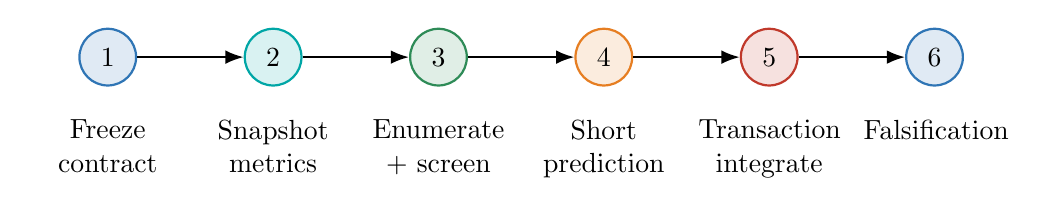
\begin{tikzpicture}[x=2.1cm,y=1cm,>=Latex]
\foreach \x/\num/\title/\col in {
0/1/Freeze contract/blue,
1/2/Snapshot metrics/cyan,
2/3/Enumerate + screen/green,
3/4/Short prediction/orange,
4/5/Transaction integrate/red,
5/6/Falsification/blue}
{
  \node[circle,fill=\col!15,draw=\col,thick,minimum size=.72cm] (n\num) at (\x,0) {\num};
  \node[align=center,text width=1.8cm,below=3mm of n\num] {\title};
}
\foreach \a/\b in {1/2,2/3,3/4,4/5,5/6}{\draw[->,thick] (n\a)--(n\b);}
\end{tikzpicture}
\vspace{1.2cm}
\begin{columns}[T,onlytextwidth]
\column{.48\textwidth}
\begin{itemize}
  \item Phase 1: state/input/base/sign/schema
  \item Phase 2: global $V,P,Q,f$, reserve, topology
  \item Phase 3: 16-action deterministic oracle
\end{itemize}
\column{.48\textwidth}
\begin{itemize}
  \item Phase 4: predictor + cost provenance
  \item Phase 5: atomic switch/rollback/fallback
  \item Phase 6: multi-event, dt/runtime sensitivity
\end{itemize}
\end{columns}
\end{frame}

\begin{frame}{14. Predeclared verification matrix}
\small
\begin{tabularx}{\textwidth}{>{\bfseries}p{.22\textwidth}XX}
\toprule
Gate & ต้องตรวจอะไร & หลักฐานผ่าน \\
\midrule
Unit/oracle & enumeration ครบและ tie-break deterministic & 16 vectors ไม่ซ้ำ, ผล repeatable \\
Metric identity & $P/Q/loss/reserve$ ใช้ base/sign ถูกต้อง & เทียบ direct KCL identities \\
Feasibility & candidate ผิด constraint ถูก reject & injected counterexamples \\
Hybrid transaction & state mapping/right-limit/rollback & no partial commit, finite residual \\
Behaviour & no-event, fault, load, SG trip/reclose & เลือก mode มีเหตุผลและไม่มี chatter \\
Numerical & $\Delta t$, horizon, finite-difference sensitivity & รายงานความต่าง ไม่ tune tolerance \\
Runtime & deadline และจำนวน candidate TDS & percentile runtime + fail-closed timeout \\
\bottomrule
\end{tabularx}
\vspace{.25cm}
\centering
\gate{ผ่านทั้งหมดก่อนเทียบ performance กับ BO}
\end{frame}

\begin{frame}{15. สิ่งที่ต้องตกลงกับอาจารย์ก่อน implement}
\begin{enumerate}
  \item นิยาม ``system recovery'' และ operating limits ที่ใช้เป็น hard constraints
  \item prediction horizon $T_p$ และ controller invocation/deadline
  \item reserve/energy model ที่อนุญาตให้ใช้จริง
  \item cost normalization และ weight provenance -- source, derived หรือ design choice
  \item safe fallback เมื่อทุก candidate ไม่ผ่าน
  \item BO ใช้เป็น baseline/offline tuner หรือไม่ และใช้ข้อมูลชุดเดียวกันอย่างไร
\end{enumerate}
\begin{alertblock}{สิ่งที่ยังไม่ควรพูด}
ยังไม่อ้างว่า ET-FCSPS มีเสถียรภาพดีกว่า BO, เร็วกว่า BO หรือเลือก GFM น้อยกว่า จนกว่าจะ implement และทดสอบบน input/event contract เดียวกัน
\end{alertblock}
\end{frame}

\begin{frame}{16. ข้อเสนอสำหรับการประชุม}
\begin{block}{One-sentence proposal}
ใช้ AGSI++ เป็น local event indicator แล้วให้ ET-FCS predictive supervisor ประเมิน mode combination ของ IBR จาก full-network feasibility และ short-horizon response ก่อน commit การสลับ
\end{block}
\begin{columns}[T,onlytextwidth]
\column{.48\textwidth}
\textbf{จุดเด่นที่คาดหวัง}
\begin{itemize}
  \item system-aware แทน threshold-only
  \item deterministic และอธิบายย้อนหลังได้
  \item enforce hard constraints ก่อนเลือก
  \item ใช้ finite set เล็กของระบบเราโดยตรง
\end{itemize}
\column{.48\textwidth}
\textbf{ความเสี่ยงที่ต้องจัดการ}
\begin{itemize}
  \item computational cost ของ prediction
  \item model mismatch และ reserve uncertainty
  \item horizon/weight sensitivity
  \item closed-loop stability ยังต้องพิสูจน์
\end{itemize}
\end{columns}
\end{frame}

\begin{frame}{แหล่งอ้างอิงหลักและขอบเขตการอ้าง}
\small
\begin{enumerate}
  \item J. Rodriguez et al., ``State of the Art of Finite Control Set Model Predictive Control in Power Electronics,'' \emph{IEEE Transactions on Industrial Informatics}, vol. 9, no. 2, pp. 1003--1016, 2013. DOI: 10.1109/TII.2012.2221469.
  \item P. I. Frazier, ``A Tutorial on Bayesian Optimization,'' arXiv:1807.02811, 2018.
  \item J. Snoek, H. Larochelle, and R. P. Adams, ``Practical Bayesian Optimization of Machine Learning Algorithms,'' \emph{NeurIPS 25}, 2012.
  \item สมการ plant, AGSI++, full-KCL และ event transaction ที่กล่าวถึงในสไลด์ อ้างจาก implementation/derivation ภายในโครงการ; ET-FCSPS เป็น \textbf{PROJECT-DERIVED PROPOSAL} ที่ยังไม่ implement
\end{enumerate}
\vspace{.4cm}
\begin{block}{ขอบเขต}
เอกสารนี้เสนอ architecture และ verification plan ไม่ใช่หลักฐานผล closed-loop ของ controller ใหม่
\end{block}
\end{frame}

\end{document}
